%\documentclass[preprint,12pt]{elsarticle}
\documentclass[review]{elsarticle}

% Use the option review to obtain double line spacing
% \documentclass[authoryear,preprint,review,12pt]{elsarticle}
%
% Use the options 1p,twocolumn; 3p; 3p,twocolumn; 5p; or 5p,twocolumn
% for a journal layout:
%\documentclass[final,1p,times]{elsarticle}
%\documentclass[final,1p,times,twocolumn]{elsarticle}
%\documentclass[final,3p,times]{elsarticle}
%\documentclass[final,3p,times,twocolumn]{elsarticle}
%\documentclass[final,5p,times]{elsarticle}
%\documentclass[final,5p,times,twocolumn]{elsarticle}

% For including figures, graphicx.sty has been loaded in
% elsarticle.cls. If you prefer to use the old commands
% please give \usepackage{epsfig}

% The amssymb package provides various useful mathematical symbols
\usepackage{amssymb}
% The amsthm package provides extended theorem environments
\usepackage{amsthm}
\usepackage{amsmath}

% Author added packages
\usepackage{url}
\usepackage{subcaption}

% The lineno packages adds line numbers. Start line numbering with
% \begin{linenumbers}, end it with \end{linenumbers}. Or switch it on
% for the whole article with \linenumbers.
%\usepackage{lineno}

\journal{Energy}

\begin{document}

\begin{frontmatter}

\title{Optimal design of energy conversion units for residential buildings}

\author{Thomas Sch\"utz\corref{mycorrespondingauthor}}
\cortext[mycorrespondingauthor]{Corresponding author}
\ead{tschuetz@eonerc.rwth-aachen.de}

\author{Markus Schraven\corref{cor2}}
\author{Julia Granacher\corref{cor2}}
\author{Dominik Kemetm\"uller\corref{cor2}}
\author{Marcus Fuchs\corref{cor2}}
\author{Dirk M\"uller\corref{cor2}}

\address{RWTH Aachen University, E.ON Energy Research Center, Institute for Energy Efficient Buildings and Indoor Climate, Mathieustr. 10, Aachen, Germany}

\begin{abstract}
%The optimal design of buildings is a complex task involving energy systems as well as construction measures.
Typically, in exact optimization models, only energy systems are considered, whereas envelope components are neglected.
When considering both, heuristics are commonly used, which do not guarantee optimal or close to optimal results.

Thus, this paper presents the governing equations, validation and exemplary usage of a building model suitable for exact optimization problems.
The developed model simultaneously considers energy systems and building envelopes.
It is based on ISO 13790 and verified according to ASHRAE 140 and further compared to a more detailed model.
The findings show that the developed model largely complies with the ASHRAE requirements and is able to assess buildings' dynamic behavior regarding indoor air temperatures as well as hourly, peak load, and annual heating and cooling loads.

The simultaneous optimization of energy system and envelope is further demonstrated analyzing retrofitting options of a residential building.
We consider solely installing additional PV units, modernizing the building envelope according to German regulations and an optimization without constraints regarding building envelope and energy system.
The results indicate that installing additional PV units can moderately reduce total costs and CO$_2$ emissions.
The envelope modernization according to governmental regulations leads to largely increased costs at lower emissions, whereas the unconstrained optimization is able to simultaneously achieve significant cost and CO$_2$ emission advantages.

\end{abstract}

\begin{keyword}
Building Energy Systems \sep German regulations \sep Mixed-Integer Linear Programming \sep Optimal Design
\end{keyword}

\end{frontmatter}

%\linenumbers

% main text
%\input{chapters/nomenclature.tex}
\section{Introduction}

The transition towards a more energy efficient and environmentally friendly economy is a recognized objective of the European Union \cite{TheEuropeanParliamentandtheCouncil2010}.
In Germany, this concept is known as ``Energiewende'' and aims at reducing greenhouse gas emissions, increasing electricity generation from renewable energy sources (RES) and achieving higher energy efficiency in general \cite{FederalMinistryforEconomicAffairsandEnergy2012}. 
In the context of buildings, which account for approximately 40\% of total energy consumption in the European Union \cite{TheEuropeanParliamentandtheCouncil2010}, emission reductions and energy savings can for example be achieved by installing more efficient heating devices and by improving their control strategy.

In recent years, many different heat and electricity generation as well as storage technologies evolved for application in buildings.
Small scale Combined Heat and Power (CHP) units offer a highly efficient method for generating heat and electricity simultaneously from fossil fuels \cite{Maghanki2013,Peacock2005}.
Potential benefits can further be leveraged by introduction of Thermal Energy Storage (TES) devices \cite{Haeseldonckx2007}.
Heat Pump (HP) systems present a technology for efficiently using electricity for heating purposes \cite{Staffell2012}.
Renewable Energy Sources (RES), especially solar systems can also be used on building level, such as for example Solar Thermal Collectors (STCs) \cite{Kalogirou2004} or Photovoltaic (PV) modules \cite{Parida2011}.
The integration of such fluctuating generators can for example be enhanced by storage devices such as TES \cite{Tian2013} and batteries \cite{Luthander2015}.

In order to achieve the proposed emission reductions and energy savings, the German government supports the utilization of environmentally friendly technologies such as RES and CHP in the building sector.
For example, the Renewable Energy Sources Act \cite{EEG2014}, guarantees above market and long-term feed-in tariffs for PV plants.
Additionally, the Combined Heat and Power Act \cite{KWKG2016} provides subsidies for feed-in and self-consumed electricity from CHP.
Further methods for promoting RES and eco-friendly technologies include subsidies from the German Reconstruction Credit Institute for combined PV and battery systems \cite{KfW275_2016} as well as private utility companies offering reduced electricity tariffs for heat pump (HP) systems.

The vast quantity of combinations of available devices into a Building Energy System (BES) requires a systematic analysis and evaluation method \cite{Yang2015}, making optimization approaches a viable option for determining the optimal structure, sizing and operation of BES.
The inherent nonlinearities arising in such optimization models, like the typically nonlinear part load behavior of generation units, led to the development of mixed-integer nonlinear programs (MINLP) \cite{Pruitt2013,Ren2008}.
However, the majority of analyses dealing with the optimal design and operation of BES consider mixed-integer linear programs (MILP), often requiring large simplifications.
These simplifications most frequently occur regarding the devices' capacity and their part load behavior.
For example, Ashouri et al. \cite{Ashouri2013} presented a MILP framework for the optimal selection and sizing of smart building systems considering all aforementioned generation and storage units, as well as chillers and ice storage systems. 
Their device modeling considers continuous equipment sizes rather than available, discrete sizes.
Furthermore, no switching on threshold or decreased part load performance are modeled.
Other studies \cite{Ameri2016,Voll2013} use the continuous dimensioning as done by Ashouri et al. \cite{Ashouri2013}, however accounting for linear part load losses.
Ameri and Besharati \cite{Ameri2016} optimize district heating and cooling networks considering gas turbines, boilers, chillers and PV.
Voll et al. \cite{Voll2013} compute an optimal energy system for industrial applications comprising CHPs, boilers and chillers.
Mehleri et al. \cite{Mehleri2012,Mehleri2013} model some equipment sizes, such as boilers, PV area and TES volume with continuous variables, whereas the CHP capacity is described with discrete steps.
They also neither account for switching on thresholds nor part load deterioration.
Their model is applied to optimize local neighborhoods considering CHPs, boilers, PV, TES and district heating as well as microgrids.
Such a mixed modeling of device capacities is further used by \cite{Harb2016,Lozano2010}.
Harb et al. \cite{Harb2016} model CHP and HP capacities discretely and rely on the continuous sizing for PV, boilers and TES.
In this model, CHP part load is handled with an empirical model, whereas constant efficiencies are assumed for HP and boilers for the entire modulation range.
The model is applied to determine optimal configurations for German residential buildings and extended to compute local heating networks and microgrids for a small neighborhood.
To the best of our knowledge, this approach presents the only available model for considering multiple electricity tariffs during the design optimization, in particular a special heat pump tariff and a standard electricity tariff.
Lozano et al. \cite{Lozano2010} present the optimization of combined heat, cooling and power systems considering CHP, boilers, chillers and TES.
They model device capacities discretely but TES sizes continuously.
Their devices are assumed to be 2-point controlled, not modeling part load.
Buoro et al. \cite{Buoro2012} analyze standard and domotic homes by optimizing their respective energy system consisting of CHP, boiler, chiller, PV, STC and TES.
The part load is based on a linear regression without accounting for the devices' activation threshold.
Renaldi et al. \cite{Renaldi2016} describe a framework for optimizing HP and TES systems for residential buildings.
Their devices' selection is entirely based on discrete choices, however their TES model assumes permanent losses for each device, even if the storage is totally discharged.
Heat pumps' temperature dependent COP is modeled, however the COP's deterioration during part load is neglected.
Wakui and Yokoyama \cite{Wakui2014} present a model for optimizing energy systems for residential buildings comprising CHP, TES, boiler and electrical water heaters.
The selection of CHP and storage tanks is coupled, so that if a certain CHP unit is chosen, a pre-specified storage tank is also installed as well.
Part load behavior is described by means of piecewise linearization, introducing multiple linear relationships that model the nonlinear part load curves.
This model has been extended in \cite{Wakui2016} by further considering HP units.
The selection of TES units has been decoupled from the selection of CHP units in this work; however, TES' sizes are chosen as a continuous variables rather than discretely.

In order to contribute to the field of optimal design of building energy systems, we present a MILP framework for determining the design, size and operation of building energy systems comprising CHP, HP, boiler, electrical heaters, TES, batteries, PV and STC.
Based on the previously described works, our paper presents three novelties.
First, we model the selection of all devices, including TES, discretely.
In this way, we assure that the determined, optimal system is available for purchase in reality, and we are able to include detailed information such as efficiency curves and investment costs for each type of device.
As illustrated previously by Wakui et al. \cite{Wakui2014,Wakui2016} for CHP units, we use multiple piecewise linearizations for all considered CHPs, HPs and boilers in this work.
The second novelty is a detailed modeling of many specific German regulations and market characteristics.
We account for limitations on PV feed-in based on the current Renewable Energy Act from 2014, we model the German Cogeneration Act from 2016 and consider subsidies for PV systems with batteries as well as reduced heat pump tariffs.
Our third contribution is the design decision between multiple gas and electricity tariffs.
Previous studies only accounted for a single gas and electricity rate, whereas we include the possibility of choosing more expensive eco-tariffs to analyze the trade-off between monetary costs and environmental impacts.

These novelties are of manifold importance.
Researchers benefit from a detailed decision modeling and part load description.
Regulators can investigate the effect of certain laws on rational decisions.
Practitioners can use the framework for determining optimal BES systems and analyzing trade-offs between economic and ecologic objectives.

The rest of this paper is structured as follows.
Section~\ref{sec:Modeling} describes the developed optimization model.
Afterwards, Section~\ref{sec:Case study} presents a case study in which the effects of all implemented German regulations are analyzed in detail.
Finally, the findings are summarized and an outlook for future research is given in Section~\ref{sec:Conclusions}.

The models and application described in this paper can be downloaded for free from \url{https://github.com/RWTH-EBC/BESopt}. (The currently private repository will be made public upon acceptance of this paper.)
\section{Modeling}
\label{sec:Modeling}

The structure of the considered building energy system is shown in Figure~\ref{fig:house_structure}.
Conventional heat generators such as boilers, CHP units, electrical heaters (EHs) and HPs are considered.
Furthermore, storage devices like electrical batteries (BATs) and TES units are available.
Solar generators like PV modules and STCs as well as peripheral devices like inverters are also included as possible parts of the optimal BES.
Thermal loads include space heating as well as domestic hot water.
Electrical loads describes the building's electricity consumption for lighting and electrical appliances.

\begin{figure}[h!]
	\begin{center}
		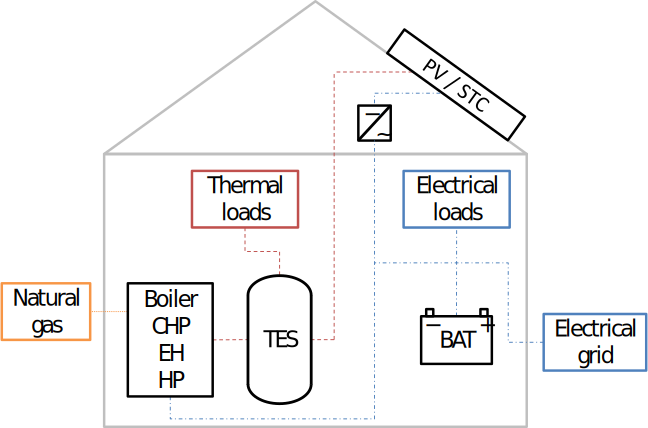
\includegraphics[width=\linewidth]{figures/house.pdf}
		\caption{Building energy system structure (single column figure)}
		\label{fig:house_structure}
	\end{center}
\end{figure}

The model requires annual inputs for these thermal and electrical loads.
Further inputs include device specific data, such as the available types (e.g. CHP unit 1, CHP unit 2, etc.) of each device (CHP, HP, etc.) and their characteristics, such as efficiency curves, expected life time, investment costs as well as operation and maintenance costs.
Also, information regarding different gas and electricity tariffs, economic parameters like interest rate, tax rates, length of the observation period and subsidy rates can be specified.

Since modeling an entire year requires long computing times, the framework also supports clustering the annual inputs into multiple representative periods that are weighted with weighting variables $\left(w_d\right)$.
The clustering is based on the k-medoids method \cite{Vinod1969,Dominguez-Munoz2011}, which has been shown to provide reliable results of high quality for energy system optimization purposes \cite{Schutz2016}.
If clustering is omitted, the weighting variables are set to 1.

The remainder of this section explains the objective functions as well as the economic, technical and ecological modeling.

\subsection{Objective functions}
The objectives of the developed model are minimization of annual costs $\left(c^\mathrm{ann}\right)$ and minimization of annual CO$_2$ emissions $\left(emi^\mathrm{ann}\right)$.
Annual costs are the sum of costs for investments $\left(c^\mathrm{inv}\right)$, operation and maintenance $\left(c^\mathrm{o\&m}\right)$, demand related costs $\left(c^\mathrm{dem}\right)$ and metering $\left(c^\mathrm{met}\right)$ less the revenues generated from feed-ins $\left(e^\mathrm{fin}\right)$ and governmental subsidies $\left(e^\mathrm{sub}\right)$.
\begin{equation}
	c^\mathrm{ann} = c^\mathrm{inv} + c^\mathrm{o\&m} + c^\mathrm{dem} + c^\mathrm{met} - e^\mathrm{fin} - e^\mathrm{sub}
	\label{eqn:obj_costs}
\end{equation}

Annual CO$_2$ emissions comprise emissions from gas usage $\left(emi^\mathrm{gas}\right)$, imported electricity $\left(emi^\mathrm{el,imp}\right)$ and negative emissions from electricity exports $\left(emi^\mathrm{el,exp}\right)$.
\begin{equation}
	emi^\mathrm{ann} = emi^\mathrm{gas} + emi^\mathrm{el,imp} - emi^\mathrm{el,exp}
\end{equation}

The following subsections describe the implemented constraints that limit the feasible search space.

\subsection{Economical constraints}
The economic modeling is based on the German engineering guideline VDI~2067 \cite{VDI_2067}, that has also been used in previous publications \cite{Harb2016,Schutz2016,Schutz2016a} \begin{LARGE}
\textbf{Applied Energy}
\end{LARGE}.

The following subsections define each element of the above mentioned parts of the economic objective.

\subsubsection{Investments}

According to this guideline, the investment costs are distributed into equal, annual payments by means of the capital recovery factor $\left(CRF\right)$.
The investment costs for each type $i$ of all devices $dev$, but PV and STC are computed as follows:
\begin{equation}
	c^\mathrm{inv}_{dev} = CRF \cdot tax^\mathrm{VAT} \cdot \sum\limits_{i} \left[ x_{dev,i} \cdot \left(1-rv_{dev,i}\right) \cdot c^\mathrm{inv}_{dev,i} \right]
\end{equation}

In this equation, $tax^\mathrm{VAT}$ represents the value added tax, $rv$ the residual value at the end of the period of interest, $c^\mathrm{inv}_{dev,i}$ the investment costs for each type of device and $x_{dev,i}$ the binary decision if type $i$ of device $dev$ is purchased or not.

For PV and STC the following equation is used, where $c^\mathrm{inv}_{dev,i}$ stands for module specific costs and $z_{dev,i}$ describes the number of installed modules of each type of collector.
\begin{equation}
	c^\mathrm{inv}_{dev} = CRF \cdot tax^\mathrm{VAT} \cdot \sum\limits_{i} \left[ z_{dev,i} \cdot \left(1-rv_{dev,i}\right) \cdot c^\mathrm{inv}_{dev,i} \right]
\end{equation}

The total investment costs mentioned in Eq.~\ref{eqn:obj_costs} are the sum of each devices' costs:
\begin{equation}
	c^\mathrm{inv} = \sum\limits_{dev} c^\mathrm{inv}_{dev}
	\label{eqn:sum_investments}
\end{equation}

The relationship shown in Eq.~\ref{eqn:sum_investments} is analogously applied to all subsequently described parts of the objective function and is therefore omitted in the following subsections.


\subsubsection{Operation and maintenance}

Costs for operation and maintenance are based on a fixed percentage $\left(f^{\mathrm{o\&m}}_{dev,i}\right)$ of the initial investment.
The corresponding values for $f^{\mathrm{o\&m}}_{dev,i}$ can be found in \cite{VDI_2067}.
For all devices but PV and STC, this relationship is modeled as:
\begin{equation}
	c^\mathrm{o\&m}_{dev} = b^{\mathrm{infl}} \cdot CRF \cdot tax^\mathrm{VAT} \cdot \sum\limits_{i} \left( x_{dev,i} \cdot c^\mathrm{inv}_{dev,i} \cdot f^{\mathrm{o\&m}}_{dev,i} \right)
	\label{eqn:costs_om_nonpvstc}
\end{equation}

In Eq.~\ref{eqn:costs_om_nonpvstc}, $b^{\mathrm{infl}}$ stands for the price dynamic cash value.
Analogously, this equation is formulated for PV and STC as follows:
\begin{equation}
	c^\mathrm{o\&m}_{dev} = b^{\mathrm{infl}} \cdot CRF \cdot tax^\mathrm{VAT} \cdot \sum\limits_{i} \left( z_{dev,i} \cdot c^\mathrm{inv}_{dev,i} \cdot f^{\mathrm{o\&m}}_{dev,i} \right)
\end{equation}

\subsubsection{Demand related costs}

Demand related costs depend on the chosen gas or electricity tariff.
If a CHP or boiler is installed, a gas tariff $\left(tar^\mathrm{gas}_{j}\right)$ has to be selected.
Furthermore, at most one gas tariff can be chosen.
\begin{align}
	\sum\limits_{j} tar^\mathrm{gas}_{j} &\ge \sum\limits_{i} x_{dev,i} \qquad \forall \; dev \in \left\lbrace\mathrm{CHP, BOI}\right\rbrace\\
	\sum\limits_{j} tar^\mathrm{gas}_{j} &\le 1
\end{align}

As many utilities offer a tiered pricing structure depending on the annual consumption, different tariff levels $\left(tar^\mathrm{gas,lvl}_{j,l}\right)$ are introduced.
At most one level can be valid and if the corresponding gas tariff is not chosen, all level variables have to be 0:
\begin{equation}
	\sum\limits_{l} tar^\mathrm{gas,lvl}_{j,l} = tar^\mathrm{gas}_{j}
\end{equation}

The correct level is bounded by a minimum annual consumption $\left(Gtar^\mathrm{LB}_{j,l}\right)$ and a maximum annual consumption $\left(Gtar^\mathrm{UB}_{j,l}\right)$:
\begin{equation}
	tar^\mathrm{gas,lvl}_{j,l} \cdot Gtar^\mathrm{LB}_{j,l} \le G^\mathrm{CHP}_{j,l} + G^\mathrm{BOI}_{j,l} \le tar^\mathrm{gas,lvl}_{j,l} \cdot Gtar^\mathrm{UB}_{j,l}
\end{equation}

In this equation, $G^\mathrm{CHP}_{j,l}$ and $G^\mathrm{BOI}_{j,l}$ describe the annual gas consumption of CHP units and boilers at tariff $j$ and level $l$.

For boilers and CHP units, the total gas consumption $G^\mathrm{tot}_{dev}$ of all days $d$ and time steps $t$ results in:
\begin{equation}
	G^\mathrm{tot}_{dev} = \sum\limits_{d} w_d \cdot \Delta t \cdot \sum\limits_{t} \sum\limits_{i} \dot{E}_{dev,i,d,t}
\end{equation}

In this equation, $\Delta t$ denotes the length of each time step, which has been set to one hour in this work.

The total gas consumption is distributed among the different levels of each tariff:
\begin{equation}
	G^\mathrm{tot}_{dev} = \sum\limits_{j} \sum\limits_{l} G^{dev}_{j,l}
\end{equation}

The demand related costs for gas consumption of boilers are computed with:
\begin{equation}
	c^{\mathrm{dem}}_{\mathrm{BOI}} = b^{\mathrm{gas}} \cdot CRF \cdot \sum\limits_{j} \sum\limits_{l} G^\mathrm{BOI}_{j,l} \cdot c^\mathrm{var,gas}_{j,l}
\end{equation}

For CHP units, a tax refund of $tax^{\mathrm{gas}}$ reduces the variable costs of $c^\mathrm{var,gas}_{j,l}$ \cite{EStG2015}:
\begin{equation}
	c^{\mathrm{dem}}_{\mathrm{CHP}} = b^{\mathrm{gas}} \cdot CRF \cdot \sum\limits_{j} \sum\limits_{l} G^\mathrm{CHP}_{j,l} \cdot \left( c^\mathrm{var,gas}_{j,l} - tax^{\mathrm{gas}} \right)
\end{equation}

Demand related electricity costs for purchases from the grid are modeled similarly to the costs for natural gas.
In contrast to the gas tariffs, at least one electricity tariff has to be chosen to satisfy plug loads:
\begin{equation}
	\sum\limits_{j^*} tar^{\mathrm{el}}_{j^*} = 1
	\label{eqn:el_tariffs plug loads}
\end{equation}

In Eq.~\ref{eqn:el_tariffs plug loads}, $j^*$ denotes all electricity tariffs that are not special heat pump tariffs.

If a heat pump is installed, a special heat pump tariff $hpt$ may be installed:
\begin{equation}
	tar^{\mathrm{el}}_{hpt} \le \sum\limits_{i} x_{i}^\mathrm{HP}
\end{equation}


Tiered pricing structures for electricity tariffs are modeled in a similar manner as for gas tariffs.
At most one level can be valid and if the corresponding electricity tariff is not chosen, all level variables have to be 0:
\begin{equation}
\sum\limits_{l} tar^\mathrm{el,lvl}_{j,l} = tar^\mathrm{el}_{j}
\end{equation}

The correct level is bounded by a minimum annual consumption $\left(Etar^\mathrm{LB}_{j,l}\right)$ and a maximum annual consumption $\left(Etar^\mathrm{UB}_{j,l}\right)$:
\begin{equation}
tar^\mathrm{el,lvl}_{j,l} \cdot Etar^\mathrm{LB}_{j,l} \le El^\mathrm{HOU}_{j,l} + El^\mathrm{HP}_{j,l} \le tar^\mathrm{el,lvl}_{j,l} \cdot Etar^\mathrm{UB}_{j,l}
\end{equation}

In this equation, $El^\mathrm{HOU}_{j,l}$ and $El^\mathrm{HP}_{j,l}$ describe the annual electricity purchases for the house's plug loads and HP at tariff $j$ and level $l$.
Since the HP tariff cannot be used to cover the house's plug loads, $El^\mathrm{HOU}_{hpt,l}$ is set to 0.

These total electricity imports are:
\begin{equation}
	El^\mathrm{tot}_{type} = \sum\limits_{d} w_d \cdot \Delta t \cdot \sum\limits_{t} \sum\limits_{i} P^{\mathrm{imp,}type}_{d,t} \qquad \forall \; type \in \left\lbrace\mathrm{HOU; HP}\right\rbrace
\end{equation}

The total amount of electricity imports is distributed among the different levels of each tariff:
\begin{equation}
	El^\mathrm{tot}_{type} = \sum\limits_{j} \sum\limits_{l} El^{type}_{j,l}
\end{equation}

Finally, the demand related costs are computed with:
\begin{equation}
c^{\mathrm{dem}}_\mathrm{el} = b^{\mathrm{el}} \cdot CRF \cdot \sum\limits_{type} \sum\limits_{j} \sum\limits_{l} El^{type}_{j,l} \cdot c^\mathrm{var,el}_{j,l}
\end{equation}

\subsubsection{Metering costs}

Metering costs directly follow from the chosen tariff and the resulting level. For gas tariffs the following equation is used:
\begin{equation}
	c^\mathrm{met}_{\mathrm{gas}} = \sum\limits_{j} \sum\limits_{l} tar^\mathrm{gas,lvl}_{j,l} \cdot c^\mathrm{fix,gas}_{j,l}
\end{equation}

In this equation, $c^\mathrm{fix,gas}_{j,l}$ denotes the fixed, annual metering costs of tariff $j$ and level $l$.
Fixed electricity metering costs are modeled analogously.

\subsubsection{Revenues from feed-in}

According to the German Renewable Energy Sources Act \cite{EEG2014}, electricity from PV is fed into the grid at a constant remuneration rate of $p^\mathrm{f-in,PV}=0.1231\,\mathrm{EUR}/\mathrm{kWh}$:
\begin{equation}
	e^\mathrm{f-in}_{\mathrm{PV}} = b^\mathrm{EEG} \cdot CRF \cdot p^\mathrm{f-in,PV} \cdot \Delta t \cdot \sum\limits_{d} \sum\limits_{t} P^{\mathrm{sell}}_{\mathrm{PV},d,t}
\end{equation}

Electricity surplus from CHP can be fed into the grid at standard market rates, which are approx. $p^\mathrm{f-in,CHP}=0.038\,\mathrm{EUR}/\mathrm{kWh}$:
\begin{equation}
	e^\mathrm{f-in}_{\mathrm{CHP}} = b^\mathrm{EEG} \cdot CRF \cdot p^\mathrm{f-in,CHP} \cdot \Delta t \cdot \sum\limits_{i} \sum\limits_{d} \sum\limits_{t} P^{\mathrm{sell}}_{\mathrm{CHP},i,d,t}
\end{equation}

\subsubsection{Subsidies}
\label{ssec:subsidies}

In this paper, we consider subsidies for CHP units according to \cite{KWKG2016} and subsidies for battery systems based on \cite{KfW275_2016}.

For large micro CHP units above 2~kW rated electrical power (subset $i^*$), the subsidies are computed as:
\begin{equation}
	e^\mathrm{sub}_{\mathrm{CHP,large}} = b^\mathrm{EEG} \cdot CRF \cdot \Delta t \cdot \sum\limits_{i^*} \sum\limits_{d} w_d \cdot \sum\limits_{t} \left[p^\mathrm{sub,CHP}_{\mathrm{self}} \cdot \left(P^\mathrm{HOU}_{\mathrm{CHP,}i^*,d,t} + P^\mathrm{HP}_{\mathrm{CHP,}i^*,d,t}\right) + p^\mathrm{sub,CHP}_{\mathrm{sell}} \cdot P^\mathrm{sell}_{\mathrm{CHP,}i^*,d,t}\right]
	\label{eqn:subs_CHP_large}
\end{equation}

In this equation, $p^\mathrm{sub,CHP}_{\mathrm{self}}=0.04\,\mathrm{EUR}/\mathrm{kWh}$ denotes the subsidies for self-consumed electricity from CHP units and $p^\mathrm{sub,CHP}_{\mathrm{sell}}=0.08\,\mathrm{EUR}/\mathrm{kWh}$ the subsidies for sold power \cite{KWKG2016}.

Smaller micro CHP units (subset $i_*$) can either receive a fixed or a variable subsidy.
The fixed subsidies are computed with:
\begin{equation}
	sub^\mathrm{fix} = CRF \cdot t^\mathrm{max} \cdot p^\mathrm{sub,CHP}_{\mathrm{fix}} \cdot \sum\limits_{i_*} x_{\mathrm{CHP,}i_*} \cdot P^\mathrm{nom}_{\mathrm{CHP,}i_*}
\end{equation}

Here, $t^\mathrm{max}$ stands for the subsidized time of 60000 hours and $p^\mathrm{sub,CHP}_{\mathrm{fix}}=0.04\,\mathrm{EUR}/\mathrm{kWh}$ is the specific subsidy.

Variable subsidies for small scale CHP units are computed just like for large scale CHPs as described in Eq.~\ref{eqn:subs_CHP_large}, however they are stored in variable $sub^\mathrm{var}$.
Since the maximum of both, $sub^\mathrm{fix}$ and $sub^\mathrm{var}$ will be used by investors, the following equations model $e^\mathrm{sub}_{\mathrm{CHP,small}} = \max\left\lbrace sub^\mathrm{fix}; sub^\mathrm{var} \right\rbrace$ in a linear manner \cite{Williams2013}.
\begin{align}
	e^\mathrm{sub}_{\mathrm{CHP,small}} &\ge sub^\mathrm{fix}\\
	e^\mathrm{sub}_{\mathrm{CHP,small}} &\ge sub^\mathrm{var}\\
	e^\mathrm{sub}_{\mathrm{CHP,small}} &\le sub^\mathrm{fix} + M^\mathrm{fix} \cdot \delta^\mathrm{var}\\
	e^\mathrm{sub}_{\mathrm{CHP,small}} &\le sub^\mathrm{var} + M^\mathrm{var} \cdot \left(1 - \delta^\mathrm{var} \right)
\end{align}

In this set of equations, $M^\mathrm{fix} = CRF \cdot t^\mathrm{max} \cdot p^\mathrm{sub,CHP}_{\mathrm{fix}} \cdot 2\,\mathrm{kW}$ is an upper bound for the fixed subsidies, $M^\mathrm{var} = b^\mathrm{EEG} \cdot CRF \cdot 8760\,\mathrm{h} \cdot p^\mathrm{sub,CHP}_{\mathrm{sell}} \cdot 2\,\mathrm{kW}$ for the variable subsidies and $\delta^\mathrm{var}$ denotes a binary variable that is 1 if the variable subsidy option is chosen.

The overall subsidies for CHP units result in:
\begin{equation}
	e^\mathrm{sub}_{\mathrm{CHP}} = e^\mathrm{sub}_{\mathrm{CHP,small}} + e^\mathrm{sub}_{\mathrm{CHP,large}}
\end{equation}

Batteries are subsidized by the German Reconstruction Credit Institute \cite{KfW275_2016}.
This subsidy is essentially a relatively cheap credit, however only 75\% of this credit have to be repaid.
Therefore, we consider 25\% of this credit as a subsidy for battery storages.
The subsidies are capped by the actual investments less $sub_{\mathrm{BAT}}=1600\,\mathrm{EUR}/\mathrm{kW}$ times the installed peak PV power, and a maximum specific amount of $sub^\mathrm{max}_\mathrm{BAT}=2000\,\mathrm{EUR}/\mathrm{kW}$:
\begin{align}
	e^\mathrm{sub}_{\mathrm{BAT}} &\le 0.25 \cdot CRF \cdot sub^\mathrm{max}_\mathrm{BAT} \cdot \zeta^\mathrm{sub}_{\mathrm{BAT}}\\
	e^\mathrm{sub}_{\mathrm{BAT}} &\le 0.25 \cdot \left(c^\mathrm{inv}_{\mathrm{PV}} + c^\mathrm{inv}_{\mathrm{BAT}} - CRF \cdot sub_{\mathrm{BAT}} \cdot \zeta^\mathrm{sub}_{\mathrm{BAT}} \right) 
\end{align}

In this set of equations, $\zeta^\mathrm{sub}_{\mathrm{BAT}}$ stands for the product of installed PV power and the decision if a battery storage is installed.
According to Williams \cite{Williams2013}, this product is linearized as follows:
\begin{align}
	\zeta^\mathrm{sub}_{\mathrm{BAT}} &\le \sum\limits_{i} P^\mathrm{nom}_{\mathrm{PV},i} \cdot z_{\mathrm{PV,}i}\\
	\zeta^\mathrm{sub}_{\mathrm{BAT}} &\le \max_j\left\lbrace P^\mathrm{nom}_{\mathrm{PV,}j} \cdot \dfrac{A^\mathrm{max}}{A_{\mathrm{PV,}j}} \right\rbrace \cdot \sum\limits_{i} x_{\mathrm{BAT,}i}\\
	\zeta^\mathrm{sub}_{\mathrm{BAT}} &\ge \sum\limits_{i} P^\mathrm{nom}_{\mathrm{PV},i} \cdot z_{\mathrm{PV,}i} - \left(1 - \sum\limits_{i} x_{\mathrm{BAT,}i}\right) \cdot \max_j\left\lbrace P^\mathrm{nom}_{\mathrm{PV,}j} \cdot \dfrac{A^\mathrm{max}}{A_{\mathrm{PV,}j}} \right\rbrace
\end{align}

\subsection{Technical constraints}

The technical constraints comprise the device selection and their operation.

\subsubsection{Device selection}

At most one unit of each device (CHP, HP, etc.) can be chosen:
\begin{equation}
	\sum\limits_{i} x_{dev,i} \le 1
\end{equation}

For PV and STC, multiple modules $\left(z_{dev,i}\right)$ of each type may be chosen, as long as the available roof-top area $\left(A^\mathrm{max}\right)$ is not exceeded.
\begin{align}
	z_{dev,i} &\le x_{dev,i} \cdot \dfrac{A^\mathrm{max}}{A_{dev,i}}\\
	\sum\limits_{dev}\sum\limits_{i} z_{dev,i} \cdot A_{dev,i} &\le A^\mathrm{max}
\end{align}

The nominal heat provided by CHP, EH, boiler and HP has to exceed the design heat load (DHL) to ensure thermal comfort during cold weather conditions:
\begin{equation}
	\sum\limits_{i} \left(x_{dev,i} \cdot \dot{Q}^\mathrm{nom}_{dev,i}\right) \ge \dot{Q}^\mathrm{DHL}
\end{equation}

\subsubsection{Device operation}

Heating devices, such as boiler, CHP units, HP units and electrical heaters, can only be switched on, if they have been purchased.
The activation is modeled with a binary variable $y_{dev,i,d,t}$ that equals 1 if type $i$ of device $dev$ is activated during time step $t$ of day $d$:
\begin{equation}
	y_{dev,i,d,t} \le x_{dev,i}
\end{equation}

We use information regarding electricity consumption or generation $\left(P^\mathrm{mds}_{dev,i,d,t,k}\right)$, fuel input $\left(\dot{E}^\mathrm{mds}_{dev,i,d,t,k}\right)$ and heat output $\left(\dot{Q}^\mathrm{mds}_{dev,i,d,t,k}\right)$ provided in manufacturer's data sheets (mds) for each device to model the part load behavior.
As air-water heat pumps' efficiencies depend on outer conditions, time indexes ($d,t$) are necessary.
Index $k$ describes the node points of the provided performance charts of each device, where $k=0$ stands for the minimum part load and $k=K$ for nominal operation.

The following set of equations describes a piecewise linearization of the performance charts:
\begin{align}
	\dot{Q}_{dev,i,d,t} &= \sum\limits_{k} w_{dev,i,d,t,k} \cdot \dot{Q}^\mathrm{mds}_{dev,i,d,t,k}\\
	\dot{E}_{dev,i,d,t} &= \sum\limits_{k} w_{dev,i,d,t,k} \cdot \dot{E}^\mathrm{mds}_{dev,i,d,t,k}\\
	P_{dev,i,d,t} &= \sum\limits_{k} w_{dev,i,d,t,k} \cdot P^\mathrm{mds}_{dev,i,d,t,k}\\
	y_{dev,i,d,t} &= \sum\limits_{k} w_{dev,i,d,t,k}
\end{align}

The weighting variables $w_{dev,i,d,t,k}$ are either continuous variables for devices with free modulation range or binary variables for discrete part load stages.
Furthermore, $w_{dev,i,d,t,k}$ form a so called Special Order Set 2 (SOS2) that implies that at most two neighboring entries within $w_{dev,i,d,t,k}$ can be greater than zero at each time step \cite{Williams2013}.
The solver used in our simulations supports SOS2, however the SOS2 relationship can easily be reformulated by introducing additional binary variables \cite{Williams2013}.

The heat output of STC is:
\begin{equation}
	\dot{Q}_{\mathrm{STC,}i,d,t} = \eta_{\mathrm{STC,}i,d,t} \cdot z_{\mathrm{STC,}i} \cdot A_{\mathrm{STC,}i} \cdot I_{d,t}
\end{equation}

Where $\eta_{\mathrm{STC,}i,d,t}$ describes the device's efficiency based on the optical efficiency as well as linear and quadratic thermal losses.
The solar irradiation onto the collector is $I_{d,t}$ and is computed according to \cite{Duffie2013,Perez1990}.

The electricity generation from PV is modeled similarly, considering the average efficiency of inverters $\left(\eta_{\mathrm{INV}}\right)$:
\begin{equation}
	P_{\mathrm{PV,}i,d,t} = \eta_{\mathrm{PV,}i,d,t} \cdot z_{\mathrm{PV,}i} \cdot A_{\mathrm{PV,}i} \cdot I_{d,t} \cdot \eta_{\mathrm{INV}}
\end{equation}

The power from PV, CHP and the power discharging the BAT is split into self-consumption for general plug loads (HOU), the HP and electricity fed into the grid (sell).
For BAT and PV, these parts can be combined for all types of modules and batteries:
\begin{equation}
	\sum\limits_{i} P_{dev,i,d,t} = P^\mathrm{HOU}_{dev,d,t} + P^\mathrm{HP}_{dev,d,t} + P^\mathrm{sell}_{dev,d,t}
\end{equation}

In case of CHP units, a strict distinction between each type of CHP has to be made due to the precise modeling of CHP subsidies:
\begin{equation}
P_{\mathrm{CHP,}i,d,t} = P^\mathrm{HOU}_{\mathrm{CHP,}i,d,t} + P^\mathrm{HP}_{\mathrm{CHP,}i,d,t} + P^\mathrm{sell}_{\mathrm{CHP,}i,d,t}
\end{equation}

According to the German Renewable Energy Sources Act \cite{EEG2014}, at most 70\% of the generated PV power may be fed into the public grid.
If a battery system is installed and the subsidies described in Section~\ref{ssec:subsidies} are chosen, this number is even reduced to 50\% \cite{KfW275_2016}.
\begin{equation}
	P^\mathrm{sell}_{\mathrm{PV,}d,t} \le \sum\limits_{i} P^\mathrm{nom}_{\mathrm{PV,}i} \left[ 0.7 \cdot \left(z_{\mathrm{PV,}i} - \zeta^{\mathrm{PV,BAT}}_i \right) + 0.5 \cdot \zeta^{\mathrm{PV,BAT}}_i \right]
	\label{eqn:limit feed in}
\end{equation}

In Eq.~\ref{eqn:limit feed in}, $\zeta^{\mathrm{PV,BAT}}_i$ stands for the product of $z_{\mathrm{PV,}i}$ and $\sum\limits_{j} x_{\mathrm{BAT,}j}$ that is linearized as follows:
\begin{align}
	\zeta^{\mathrm{PV,BAT}}_i &\le z_{\mathrm{PV,}i}\\
	\zeta^{\mathrm{PV,BAT}}_i &\le \dfrac{A^{\mathrm{max}}}{A_{\mathrm{PV,}i}} \cdot \sum\limits_{j} x_{\mathrm{BAT,}j}\\
	\zeta^{\mathrm{PV,BAT}}_i &\ge z_{\mathrm{PV,}i} - \left(1- \sum\limits_{j} x_{\mathrm{BAT,}j}\right) \cdot \dfrac{A^{\mathrm{max}}}{A_{\mathrm{PV,}i}}
\end{align}

The inverter is sized according to the installed, nominal PV power:
\begin{equation}
	\sum\limits_{i} z_{\mathrm{PV,}i} \cdot P^\mathrm{nom}_{\mathrm{PV,}i} \le \sum\limits_{j} x_{\mathrm{INV,}j} \cdot P^\mathrm{nom}_{\mathrm{INV,}j}
\end{equation}

Storage units' energy contents are modeled based on their state of charge $S_{dev,i,d,t}$.
The state of charge can only be positive, if the corresponding device has been purchased:
\begin{equation}
	S_{dev,i,d,t} \le x_{dev,i}
\end{equation}

In order to allow a discrete selection of storage units, an energy balance is modeled for each type:
\begin{equation}
	S_{dev,i,d,t} = \left(1-\varphi_{dev,i}\right) \cdot S_{dev,i,d,t-1} + \Delta t \cdot \dfrac{\eta_{dev_i} \cdot ch_{dev,i,d,t} - dch_{dev,i,d,t}}{cap_{dev,i}}
	\label{eqn:soc_storages}
\end{equation}

The storage's relative standby losses between two consecutive time steps are $\varphi_{dev,i}$, $\eta_{dev_i}$ describes the storage cycle's efficiency, $ch_{dev,i,d,t}$ and $dch_{dev,i,d,t}$ stand for the charging and discharging energy and $cap_{dev,i}$ for the storage's capacity.
The capacity can be directly derived from data sheets for BATs.
For TES units, we calculate $cap_{dev,i}=\rho \cdot \kappa\cdot V_i \cdot \Delta T^\mathrm{max}$, where $\rho$ and $\kappa$ are the density and specific heat capacity of water, $V_i$ is the storage's volume and $\Delta T^\mathrm{max}=40\,\mathrm{K}$ the maximum temperature spread inside the tank.
Charging and discharging energy are restricted with big-M formulations, preventing the charging and discharging of tanks that have not been installed.
Appropriate bounds for BATs can be derived from data sheets and multiples of the design heat load are used for TES units.

For TES units, the following balances are applied to determine the charging and discharging energies:
\begin{align}
	\sum\limits_{i} ch_{\mathrm{TES,}i,d,t} &= \sum\limits_{dev^*} \sum\limits_{j} \dot{Q}_{dev^*,j,d,t}\\
	\sum\limits_{i} dch_{\mathrm{TES,}i,d,t} &= \dot{Q}^\mathrm{DHW}_{d,t} + \dot{Q}^\mathrm{SH}_{d,t}
\end{align}

In these formulations, $dev^*$ describes the subsets of all heat generating devices, $\dot{Q}^\mathrm{DHW}_{d,t}$ and $\dot{Q}^\mathrm{SH}_{d,t}$ describe the building's domestic how water and space heating demands at time $t$ on day $d$.
Both equations, in combination with the big-M constraints, ensure that all generated and demanded heat are interchanged with exactly one storage tank, nullifying all but one of the relationships presented in Eq.~\ref{eqn:soc_storages}

For BAT systems, the charging and discharging powers follow from the building's electricity balances.
We formulate one balance for the building's plug loads and a second balance for the electricity potentially billed with a special heat pump tariff.
The building's electricity balance is written as:
\begin{equation}
	P^\mathrm{HOU}_{d,t} + P^\mathrm{HOU}_{\mathrm{EH,}d,t} + \sum\limits_{i} ch_{\mathrm{BAT,}i,d,t} = P^\mathrm{imp,HOU}_{d,t} + P^\mathrm{HOU}_{\mathrm{PV,}d,t} + P^\mathrm{HOU}_{\mathrm{BAT,}d,t} + \sum\limits_{i} P^\mathrm{HOU}_{\mathrm{CHP,}i,d,t}
\end{equation}

Here, $P^\mathrm{HOU}_{d,t}$ describes the house's plug loads and $P^\mathrm{HOU}_{\mathrm{EH,}d,t}$ the amount of electricity provided by an EH that is not billed under a special heat pump tariff.

The second electricity balance is:
\begin{equation}
	\sum\limits_{i} P_{\mathrm{HP,}i,d,t} + P^\mathrm{HP}_{\mathrm{EH,}d,t} = P^\mathrm{imp,HP}_{d,t} + P^\mathrm{HP}_{\mathrm{PV,}d,t} + P^\mathrm{HP}_{\mathrm{BAT,}d,t} + \sum\limits_{i} P^\mathrm{HP}_{\mathrm{CHP,}i,d,t}
\end{equation}

The EHs electricity amounts are further described:
In total, the amount of electricity purchased at a potential heat pump tariff and the amount purchased at the standard tariff, have to be equal to the electricity consumption caused by this device:
\begin{equation}
	\sum\limits_{i} P_{\mathrm{EH,}i,d,t} = P^\mathrm{HOU}_{\mathrm{EH,}d,t} + P^\mathrm{HP}_{\mathrm{EH,}d,t}
\end{equation}

If no heat pump has been purchased, the electrical heater cannot be active in the second electricity balance:
\begin{equation}
	P^\mathrm{HP}_{\mathrm{EH,}d,t} \le \max_j\left\lbrace P^\mathrm{nom}_{\mathrm{EH},j} \right\rbrace \cdot \sum\limits_{i}x_{\mathrm{HP,}i}
\end{equation}

Finally, we prevent the heat pump from being activated if the storage temperature is above the heat pump's maximum flow temperature:
\begin{equation}
	\sum\limits_{i} S_{\mathrm{TES,}i,d,t} \le 1 - y_{\mathrm{HP,}j,d,t} \cdot \left( 1 - \dfrac{\Delta T^\mathrm{HP}}{\Delta T^\mathrm{max}} \right)
\end{equation}


\subsection{Ecological constraints}
We consider emissions from gas consumption and electricity purchase from the distribution grid as well as negative emissions for exporting electricity to the grid.

Considering the specific CO$_2$ emissions $\left(emi^\mathrm{gas,spec}_{j}\right)$ for each tariff $j$, the emissions from natural gas result in:
\begin{equation}
	emi^\mathrm{gas} = \sum\limits_{j} emi^\mathrm{gas,spec}_{j} \cdot \sum\limits_{l}  \left(G^\mathrm{CHP}_{j,l} + G^\mathrm{BOI}_{j,l}\right)
\end{equation}

Similarly, CO$_2$ emissions from electricity imports are modeled:
\begin{equation}
	emi^\mathrm{el,imp} = \sum\limits_{j} emi^\mathrm{el,spec}_{j} \cdot \sum\limits_{l} \left(El^\mathrm{HOU}_{j,l} + El^\mathrm{HP}_{j,l}\right)
\end{equation}

For computing negative emissions from electricity exports, we first compute the entire amount of exported electricity, $El^\mathrm{EXP,tot}$:
\begin{equation}
	El^\mathrm{EXP,tot} = \sum\limits_{d} w_d \cdot \Delta t \cdot \sum\limits_{t} \left[ \left( \sum\limits_{i} P_{\mathrm{CHP,}i,d,t}^\mathrm{sell} \right) + P_{\mathrm{PV},d,t}^\mathrm{sell} + P_{\mathrm{BAT,}d,t}^\mathrm{sell} \right]
\end{equation}

The following two equations ensure that electricity exports are attributed with the same CO$_2$ emissions as would occur for imports under the chosen tariff.
Since a special heat pump tariff could be selected in addition to a regular tariff, the subset $j^*$ denotes regular tariffs only.
\begin{equation}
	El^\mathrm{EXP,tot} = \sum\limits_{j^*} El^\mathrm{EXP}_{j^*}
\end{equation}
\begin{equation}
	El^\mathrm{EXP}_{j^*} \le tar_{j^*}^\mathrm{el} \cdot \max_l \left\lbrace Etar^\mathrm{UB}_{j^*,l} \right\rbrace
\end{equation}

Finally, the negative CO$_2$ emissions from electricity exports result in
\begin{equation}
	emi^\mathrm{el,exp} = \sum\limits_{j^*} emi^\mathrm{el,spec}_{j^*} \cdot El^\mathrm{EXP}_{j^*}
\end{equation}
\section{Case study}
\label{sec:Case study}

This section describes a case study in which the effects of the implemented German regulations on the optimal BES configuration as well as resulting annualized costs and emissions are analyzed.

The following subsections summarize the used inputs and the obtained results.
Further information on both as well as the implemented model can be found in this project's open-source repository\footnote{\url{https://github.com/RWTH-EBC/BESopt}}.

\subsection{Inputs}

The inputs consist of the building's energy load profiles, such as electricity demands of plug loads, domestic hot water usage and space heating loads.
Additionally, the considered energy conversion units are described in this subsection.

\subsubsection{Energy load profiles}

We applied the optimization model described in the previous section to a residential building located in Aachen (Germany) with 4 residents and a total of 255~m$^2$ heated floor area.
The hourly space heating profiles are computed with the model verified in \textbf{CITE APPLIED ENERGY PAPER}.
Electricity demands for non-heating devices, appliances and lighting are computed with a high-resolution, stochastic tool based on Richardson et al. \cite{Richardson2010}.
Domestic hot water demand profiles are computed with a combination of users' occupancy based on Richardson et al. \cite{Richardson2010} and daily tap water usage statistics of residential buildings developed in IEA Annex 42 \cite{IEAEnergyConservationinBuildingsCommunitySystems}.
The cumulated, annual space heating and domestic hot water demands result in 23500~kWh and the annual electricity demand is 4000~kWh.

\subsubsection{Energy conversion units}

All energy conversion units that have been modeled are based on manufacturers' data sheets and price recommendations from retailers or original manufacturers.
We consider between 7 and 12 different types of electrical and gas-fired heating devices.
Their ranges regarding nominal heat output and investment costs are shown in Table~\ref{tab: parameters heating devices}.
Similarly, Table~\ref{tab: parameters solar devices} summarizes the solar devices and inverters, and Table~\ref{tab: parameters storage devices} lists the ranges of storage devices.


\begin{table}[h!]
	\caption{Summary of considered heating devices}
	\centering
	\begin{tabular}[l]{@{}lccc}
		\hline
		Component 	& No. types	& $\dot{Q}^\mathrm{nom}$& $c^\mathrm{inv}$ \\
					&  			& kW 					& 1000 Euro \\
		\hline
		CHP 		& 7 		& 0.70 -- 45.00 		& 8.93 -- 62.07\\
		BOI 		& 8 		& 14.20 -- 66.30 		& 1.33 -- 4.26\\
		EH 			& 12 		& 2.00 -- 12.00 		& 0.17 -- 0.22\\
		HP 			& 8 		& 3.25 -- 50.00 		& 3.94 -- 25.44\\
		\hline
	\end{tabular}
	\label{tab: parameters heating devices}
\end{table}

\begin{table}[h!]
	\caption{Summary of solar devices and inverters}
	\centering
	\begin{tabular}[l]{@{}lccc}
		\hline
		Component 	& No. types	& $P^\mathrm{nom}$/$\dot{Q}^\mathrm{nom}$& $c^\mathrm{inv}$ \\
		&  			& kW 					& 1000 Euro \\
		\hline
		PV 			& 9 		& 0.14 -- 0.23 		& 0.16 -- 0.26\\
		STC 		& 10 		& 0.42 -- 1.32 		& 0.19 -- 0.82\\
		INV			& 27 		& 1.60 -- 28.60 	& 0.59 -- 3.67\\
		\hline
	\end{tabular}
	\label{tab: parameters solar devices}
\end{table}

\begin{table}[h!]
	\caption{Summary of storage devices}
	\centering
	\begin{tabular}[l]{@{}lccc}
		\hline
		Component 	& No. types	& Capacity 		& $c^\mathrm{inv}$ \\
					&  			& kWh / m$^3$ 	& 1000 Euro \\
		\hline
		BAT 		& 9 		& 3.60 -- 11.60		& 6.00 -- 14.33\\
		TES 		& 14 		& 0.12 -- 2.00 		& 0.42 -- 1.71\\
		\hline
	\end{tabular}
	\label{tab: parameters storage devices}
\end{table}

\subsubsection{Tariffs and emissions}

The electricity and gas tariffs' characteristics are listed in Table~\ref{tab: parameters tariffs}.
All tariffs are derived from German utility providers.
As shown in Table~\ref{tab: parameters tariffs}, standard tariffs are slightly less expensive than eco tariffs, but cause significantly more CO$_2$ emissions.
The implemented heat pump tariff further offers a strong economic incentive compared to the other tariffs.


\begin{table}[h!]
	\caption{Summary of storage devices}
	\centering
	\begin{tabular}[l]{@{}lccc}
		\hline
		Tariff 	& $c^\mathrm{fix}$	& $c^\mathrm{var}$ 		& $emi^\mathrm{spec}$ \\
		& Euro / a 	& Euro / kWh & kg CO$_2$ / kWh \\
		\hline
		Gas (standard) & \multicolumn{1}{r}{39.98 -- 182.50} & \multicolumn{1}{r}{0.080 -- 0.058} & 0.250 \\
		Gas (eco) & \multicolumn{1}{r}{39.98 -- 182.50} & \multicolumn{1}{r}{0.083 -- 0.061} & 0.238 \\
		\hline
		El. (standard) & \multicolumn{1}{r}{73.02 -- 84.16} & 0.266 -- 0.263 & 0.569 \\
		El. (eco) & \multicolumn{1}{r}{73.02 -- 117.73} & \multicolumn{1}{r}{0.275 -- 0.265} & 0.329 \\
		El. (heat pump) & \multicolumn{1}{r}{91.51}  & \multicolumn{1}{r}{0.196} & 0.508 \\
		\hline
	\end{tabular}
	\label{tab: parameters tariffs}
\end{table}

\subsection{Scenarios}

We analyze how the implemented regulations affect the optimal BES configuration, therefore we consider for each regulation one scenario in which the respective regulation is activated and a comparison in which it is deactivated.

In the \emph{PV with EEG scenario}, the solver has to install at least one PV module and simultaneously the restrictions of the Renewable Energy Sources Act, such as the fixed feed-in remuneration and limited feed-in, are enforced.
In the \emph{PV without EEG scenario}, the solver also has to install at least one PV module but neither feed-in subsidies nor limits on the PV feed-in are set.
For both scenarios, no additional constraints on the heat generation system are used, allowing the optimizer to choose any available devices.

The \emph{CHP with KWKG scenario} requires the installation of a CHP unit while accepting the subsidies according to the Cogeneration Act for feed-in and self-consumed electricity.
On the other hand, in the \emph{CHP without KWKG scenario}, the solver is forced to install a CHP unit without receiving any subsidies for electricity generated with the CHP unit.

The \emph{HP with tariff scenario} enforces the installation of a HP and choosing a special HP tariff.
In the \emph{HP without tariff scenario}, a HP is installed, but a regular electricity tariff is chosen.

Finally, the \emph{BAT with KfW scenario} analyzes the installation of a BAT with the KfW support program that provides financial incentives to lower feed-in limits of electricity generated with PV.
In the \emph{BAT without KfW scenario}, a BAT is installed, waiving the financial support through KfW but keeping the right to export electricity from PV according to the limits based on the Renewable Energy Sources Act.

Additionally, we use two different methods to compare the results in a broader context.
The first reference is the \emph{traditional scenario} forcing a traditional BES design that only allows for installing a boiler to cover the heat demand and purchasing the entire electricity demand from the grid.
While all previously mentioned scenarios minimize the total annualized costs, the second reference is the \emph{Pareto-Set} of the multi-objective optimization minimizing annualized costs and emissions.
This multi objective optimization is based on the $\varepsilon$-constraint method described by Mavrotas \cite{Mavrotas2009}.
The \emph{traditional scenario} is still a common design paradigm and the \emph{Pareto-Set} serves for assessing the economical and ecological results of the other scenarios on a global optimal scale.

These ten different scenarios are summarized in Table~\ref{tab: scenarios setup}.

\begin{table}[h!]
	\caption{Summary of investigated scenarios}
	\centering
	\begin{tabular}[l]{@{}lll}
		\hline
		Scenario 	& Device selection	& Subsidies / restrictions \\
		\hline
		PV with EEG & At least one PV module & Fixed above market feed-in remuneration\\
		& & Max. 70\% of PV peak power can be fed into the grid\\
		PV without EEG & At least one PV module & Market based feed-in remuneration\\
		& & No limitations on feed-in\\
		\hline
		CHP with KWKG & Force CHP purchase & Subsidies for feed-in and self-consumption from CHP\\
		CHP without KWKG & Force CHP purchase & No subsidies for electricity from CHP units\\
		\hline
		HP with tariff & Force HP purchase & Select reduced HP tariff\\
		HP without tariff & Force HP purchase & Prohibit reduced HP tariff\\
		\hline
		BAT with KfW & Select a BAT & Financial support according to KfW\\
		& & Max. 50\% of PV peak power can be fed into the grid\\
		BAT without KfW & Select a BAT & No financial support for BAT\\
		& & Max. 70\% of PV peak power can be fed into the grid\\
		\hline
		Traditional & Only BOI and TES & EEG, KWKG, KfW and free choice of electricity tariff \\
		Pareto-Set & No presetting &  EEG, KWKG, KfW and free choice of electricity tariff \\
		
	\end{tabular}
	\label{tab: scenarios setup}
\end{table}

\subsection{Computing hardware}

All computations are carried out with Gurobi~6.5\footnote{\url{http://www.gurobi.com/index}} and modeled with the corresponding Python framework.
We used the Branch-and-Cut \cite{Wolsey1998} algorithms from this solver.
The optimizations are solved to an optimality gap of 1\% on a Windows~7 computer with 6~CPU cores, 12~threads and 32~GB of RAM.


\subsection{Results}
\label{ssec: Results}

The resulting annualized costs and CO$_2$ emissions for all investigated scenarios are shown in Fig.~\ref{fig: pareto set}.
The full black line displays the Pareto set and the cross stands for the traditional BES design.
Circles mark the CHP scenarios, diamonds the PV scenarios, stars the forced installation of a HP and rectangles the BAT scenarios.
Red markers represent scenarios in which subsidies are considered and blue markers show the results for not using the available subsidies.
The following subsections describe the results of each scenario in more detail.

\begin{figure}[h!]
	\begin{center}
		\includegraphics[width=\linewidth]{figures/pareto_set.pdf}
		\caption{Annualized costs and emissions (single column figure)}
		\label{fig: pareto set}
	\end{center}
\end{figure}

\subsubsection{Pareto set}
The Pareto set describes all solutions in which the costs can only be reduced at the expense of increased CO$_2$ emissions, therefore no solution can simultaneously decrease costs and CO$_2$ emissions below this frontier.
The cost optimal solution, which also coincides with the PV with EEG scenario (red diamond), requires 3140~EUR and causes 2.38~tons of CO$_2$ per year.
On the other hand, the optimal solution regarding emissions, costs 8410~EUR and emits -2.68~tons of CO$_2$.
Between these two limits, we calculated five additional points to approximate the Pareto curve.

The installed rated powers of each point of the Pareto curve are displayed in Fig.~\ref{fig: heat generation moo}.
For all optimizations, a 14.2~kW boiler is chosen that functions as a primary heat generator for cost efficient solutions and as a backup unit for low emission solutions.
Additionally, small EH devices are purchased as inexpensive, electricity driven heat generators that utilize excess electricity produced from PV units.
Such PV units are installed in every point of the Pareto set.
The installed PV peak power is 11.2~kW for cost optimal solutions and increases with rising focus on emissions to 13.5~kW.
Further additions of PV are not possible due to the limited available roof area.
With increasing focus on emissions, heat is mostly generated through HP units.
Only in the minimal emissions calculation, a small CHP unit is purchased.
The only time a

\begin{figure*}[h!]
	\begin{center}
		\includegraphics[width=\linewidth]{figures/plot_cap_gen_moo.pdf}
		\caption{Rated powers (Pareto set) (double column figure)}
		\label{fig: heat generation moo}
	\end{center}
\end{figure*}

Fig.~\ref{fig: cap storage moo} shows the installed capacities of storage units.
Red bars display the water volume of TES units and blue bars the capacity of BAT.
Pure cost minimization leads to the installation of a small scale TES unit, but with increasing importance of emissions, the TES volume is increased.
The jump from approx. 0.1~m$^3$ in the cost optimal solution to 0.6~m$^3$ in optimization~1 is also due to the installation of a small scale STC unit that provides 1.9\% of the annual thermal demand.
Larger TES volumes also allow for shifting the HP's operation to times with higher PV availability, reducing grid dependency.
In the minimum emissions calculation, a large BAT system is installed allowing for even more flexible operations.

\begin{figure}[h!]
	\begin{center}
		\includegraphics[width=\linewidth]{figures/plot_cap_sto_moo.pdf}
		\caption{Capacities of storage devices (Pareto set) (single column figure)}
		\label{fig: cap storage moo}
	\end{center}
\end{figure}

The heat coverage ratios for the Pareto efficient optimizations are depicted in Fig.~\ref{fig: heat coverage moo}.
In the minimum cost case, more than 99.6\% of the annual thermal demand is covered with the boiler, the rest is generated through the backup EH.
With increasing awareness of emissions, the boiler's usage is reduced.
Initially, in optimization~1, it is marginally substituted with an STC that contributes 1.9\% of the heating demand.
After installation of a HP in optimization~2, the boiler mainly serves as a backup unit that provides approx. 10\% of the heating demand.
In the minimum emissions case, a CHP unit is installed additionally.
In this case, 99.5\% of the annual thermal demand is generated with either CHP or HP.

The self-consumption rate of electricity generated locally with either CHP or PV increases from 10\% in the most cost-efficient optimization to approx. 20\% when a HP is installed. 

\begin{figure}[h!]
	\begin{center}
		\includegraphics[width=\linewidth]{figures/plot_coverage_moo.pdf}
		\caption{Heat coverages (Pareto set) (single column figure)}
		\label{fig: heat coverage moo}
	\end{center}
\end{figure}






\subsubsection{Traditional scenario}
The black cross in Fig.~\ref{fig: pareto set} marks the result of the traditional scenario.
In comparison with the other cases, this scenario leads to the highest CO$_2$ emissions of 8.71~tons per year.
The annualized costs are 3616~EUR.
The BES consists of a 14.20~kW boiler and a TES with 0.12~m$^3$ of water volume.
Since on-site generation through PV or CHP units is prohibited, the entire electricity amount of 4000~kWh/a is bought from the distribution grid.



\subsection{PV scenarios}
In Fig.~\ref{fig: pareto set}, the diamonds represent the PV scenarios.
Red color indicates that the corresponding restrictions, in this case the subsidies according to the German Renewable Energy Sources Act, are activated, while blue markers stand for deactivated subsidies.


\subsubsection{CHP scenarios}
In Fig.~\ref{fig: pareto set}, the circles represent the CHP scenarios.
Red color indicates that the corresponding restrictions, in this case the subsidies according to the German Cogeneration Act, are activated, while blue markers stand for deactivated subsidies.
In both cases, the same BES comprising a 2.50~kW CHP unit, a 14.20~kW boiler and a 4.5~kW backup resistance heater are used to cover the thermal loads.
Furthermore, a 0.49~m$^3$ TES unit and 69.8~m$^2$ of PV area are installed.

The devices' operation is barely affected by the subsidies.
Both scenarios achieve approx. 4400 full load hours for the CHP unit and run this device electricity driven, leading to 



\begin{figure}[h!]
	\begin{center}
		\includegraphics[width=\linewidth]{figures/plot_cap_sto_other.pdf}
		\caption{Capacities of storage devices (rest) (single column figure)}
		\label{fig: cap storage other}
	\end{center}
\end{figure}



\begin{figure}[h!]
	\begin{center}
		\includegraphics[width=\linewidth]{figures/plot_coverage_other.pdf}
		\caption{Heat coverages (other) (single column figure)}
		\label{fig: heat coverage other}
	\end{center}
\end{figure}



\begin{figure*}[H!]
	\begin{center}
		\includegraphics[width=\textwidth]{figures/plot_cap_gen_other.pdf}
		\caption{Rated powers (other) (double column figure)}
		\label{fig: heat generation other}
	\end{center}
\end{figure*}
\input{chapters/conclusions.tex}
%\input{chapters/acknowledgment.tex}

\appendix

%\input{chapters/appendix.tex}

\section*{References}

\bibliographystyle{elsarticle-num} 
\bibliography{mybibfile}

\end{document}
\endinput

